\onecolumn
\appendices
\section{FSC-147 and FSC-133}
\subsection{Similar and Different Images}\label{similaranddifferent}
\begin{figure*}[!ht]
    \centering
    \fontsize{9}{9}\selectfont
    Train \\ \vspace{0.25em}
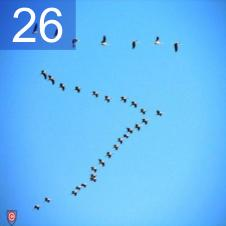
\includegraphics[height=0.15\textwidth, width=0.15\textwidth]{appendicies/numbered_ims/4399.jpg}%
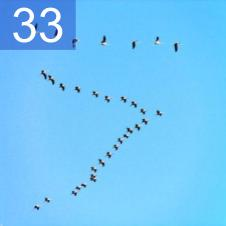
\includegraphics[height=0.15\textwidth, width=0.15\textwidth]{appendicies/numbered_ims/4620.jpg}%
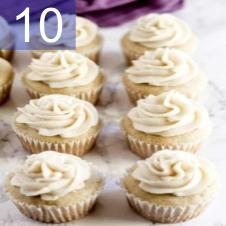
\includegraphics[height=0.15\textwidth, width=0.15\textwidth]{appendicies/numbered_ims/3812.jpg}%
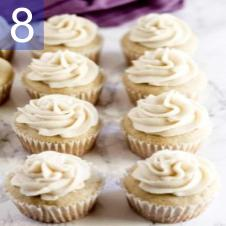
\includegraphics[height=0.15\textwidth, width=0.15\textwidth]{appendicies/numbered_ims/5238.jpg}%
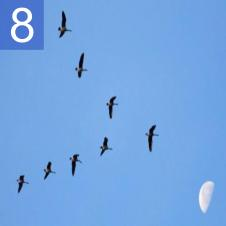
\includegraphics[height=0.15\textwidth, width=0.15\textwidth]{appendicies/numbered_ims/6684.jpg}%
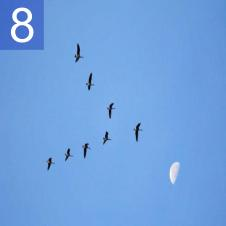
\includegraphics[height=0.15\textwidth,
width=0.15\textwidth]{appendicies/numbered_ims/4350.jpg}%
\\
\vspace{-0.5em}

\includegraphics[height=0.15\textwidth, width=0.15\textwidth]{appendicies/numbered_ims/3462.jpg}%
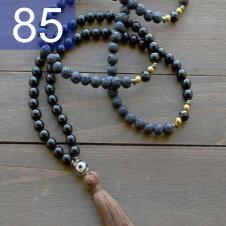
\includegraphics[height=0.15\textwidth, width=0.15\textwidth]{appendicies/numbered_ims/5638.jpg}%
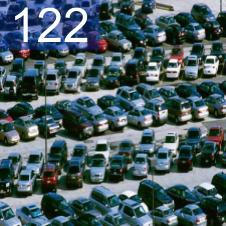
\includegraphics[height=0.15\textwidth, width=0.15\textwidth]{appendicies/numbered_ims/6138.jpg}%
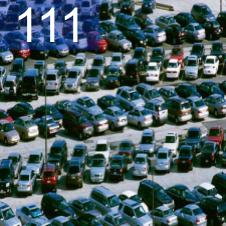
\includegraphics[height=0.15\textwidth, width=0.15\textwidth]{appendicies/numbered_ims/6864.jpg}%
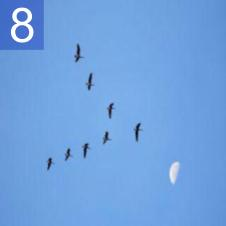
\includegraphics[height=0.15\textwidth, width=0.15\textwidth]{appendicies/numbered_ims/4707.jpg}%
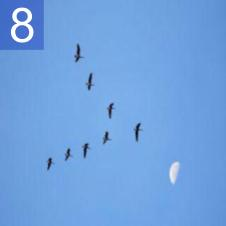
\includegraphics[height=0.15\textwidth, width=0.15\textwidth]{appendicies/numbered_ims/4683.jpg}%
\\
\vspace{-0.5em}
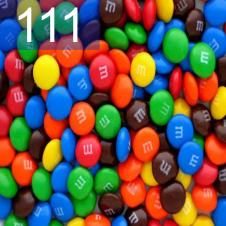
\includegraphics[height=0.15\textwidth, width=0.15\textwidth]{appendicies/numbered_ims/3506.jpg}%
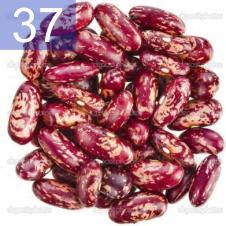
\includegraphics[height=0.15\textwidth, width=0.15\textwidth]{appendicies/numbered_ims/3791.jpg}%
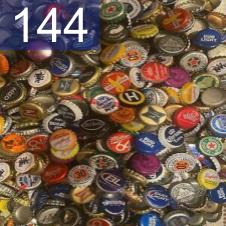
\includegraphics[height=0.15\textwidth, width=0.15\textwidth]{appendicies/numbered_ims/2891.jpg}%
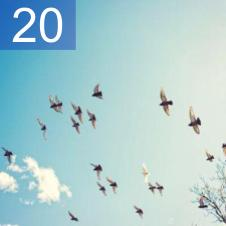
\includegraphics[height=0.15\textwidth, width=0.15\textwidth]{appendicies/numbered_ims/4386.jpg}%
% } & 
% \subfloat[21]{
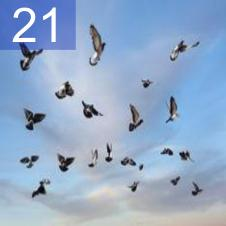
\includegraphics[height=0.15\textwidth, width=0.15\textwidth]{appendicies/numbered_ims/6567.jpg}%
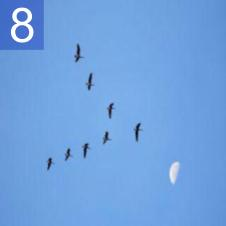
\includegraphics[height=0.15\textwidth, width=0.15\textwidth]{appendicies/numbered_ims/4375.jpg}%
\\
Val \\ \vspace{0.25em}
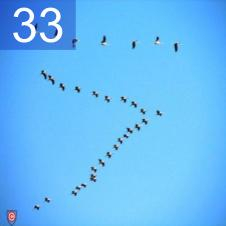
\includegraphics[height=0.15\textwidth, width=0.15\textwidth]{appendicies/numbered_ims/4549.jpg}%
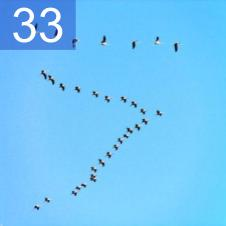
\includegraphics[height=0.15\textwidth, width=0.15\textwidth]{appendicies/numbered_ims/4719.jpg}%
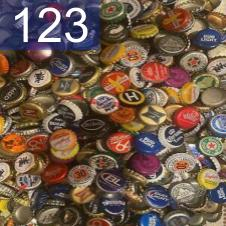
\includegraphics[height=0.15\textwidth, width=0.15\textwidth]{appendicies/numbered_ims/1896.jpg}%
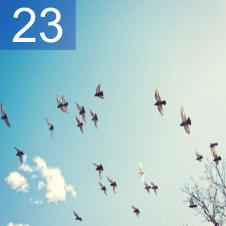
\includegraphics[height=0.15\textwidth, width=0.15\textwidth]{appendicies/numbered_ims/7415.jpg}%
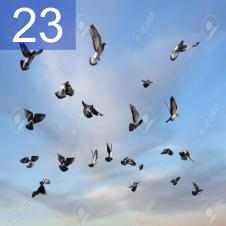
\includegraphics[height=0.15\textwidth, width=0.15\textwidth]{appendicies/numbered_ims/929.jpg}%
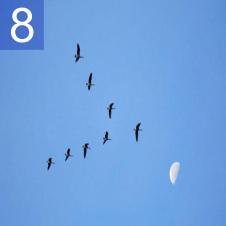
\includegraphics[height=0.15\textwidth, width=0.15\textwidth]{appendicies/numbered_ims/4704.jpg}%
\\
Test \\ \vspace{0.25em}
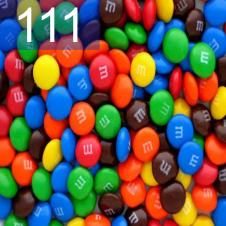
\includegraphics[height=0.15\textwidth, width=0.15\textwidth]{appendicies/numbered_ims/3698.jpg}%
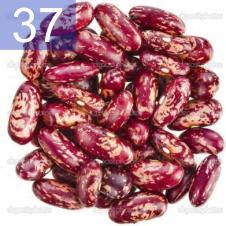
\includegraphics[height=0.15\textwidth, width=0.15\textwidth]{appendicies/numbered_ims/3494.jpg}%
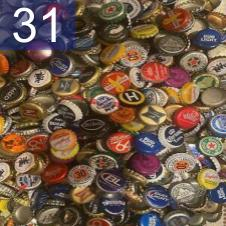
\includegraphics[height=0.15\textwidth, width=0.15\textwidth]{appendicies/numbered_ims/3282.jpg}%
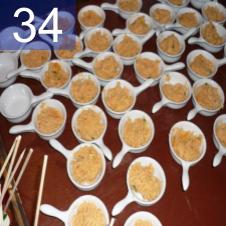
\includegraphics[height=0.15\textwidth, width=0.15\textwidth]{appendicies/numbered_ims/3285.jpg}%
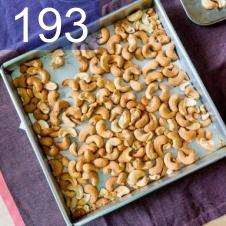
\includegraphics[height=0.15\textwidth, width=0.15\textwidth]{appendicies/numbered_ims/5142.jpg}%
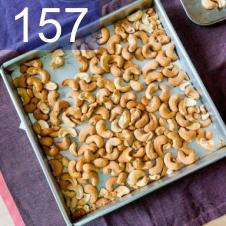
\includegraphics[height=0.15\textwidth, width=0.15\textwidth]{appendicies/numbered_ims/5801.jpg}%

    \caption{Examples of some of the 448 identical or close to identical images that appear in FSC-147 with different image IDs and their associated `ground truth' counts . Duplicates can occur with different count labels and/or in different splits.}
    \label{subset_dupes}
\end{figure*}

\begin{figure*}[!ht]   
    \centering
    \fontsize{9}{9}\selectfont
    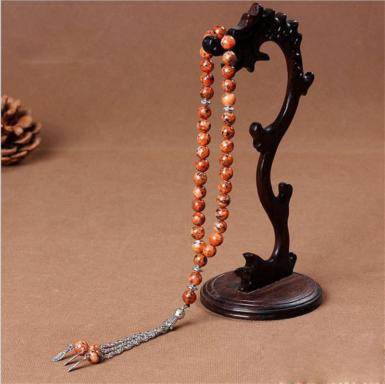
\includegraphics[height=0.19\linewidth,width=0.19\linewidth]{appendicies/raw_ims/6395.jpg}%
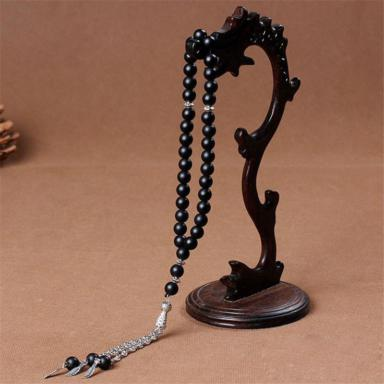
\includegraphics[height=0.19\linewidth,width=0.19\linewidth]{appendicies/raw_ims/6433.jpg}%
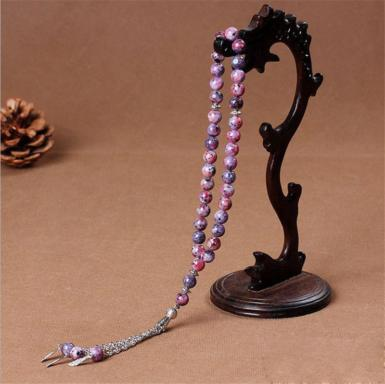
\includegraphics[height=0.19\linewidth,width=0.19\linewidth]{appendicies/raw_ims/6455.jpg}%
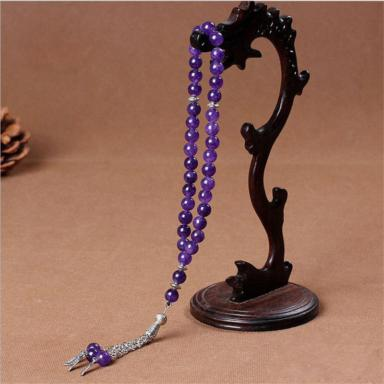
\includegraphics[height=0.19\linewidth,width=0.19\linewidth]{appendicies/raw_ims/6465.jpg}%
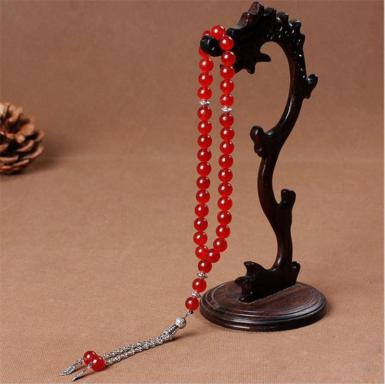
\includegraphics[height=0.19\linewidth,width=0.19\linewidth]{appendicies/raw_ims/6544.jpg}%
\\
\vspace{-0.15em}
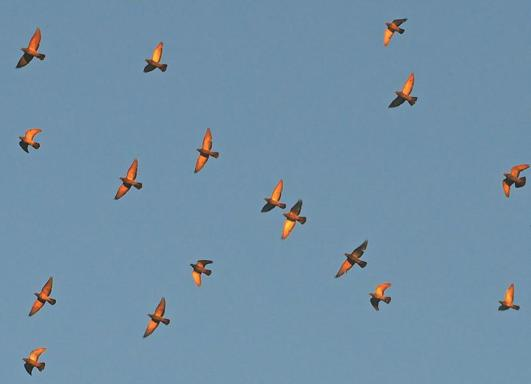
\includegraphics[height=0.19\linewidth,width=0.19\linewidth]{appendicies/raw_ims/396.jpg}%
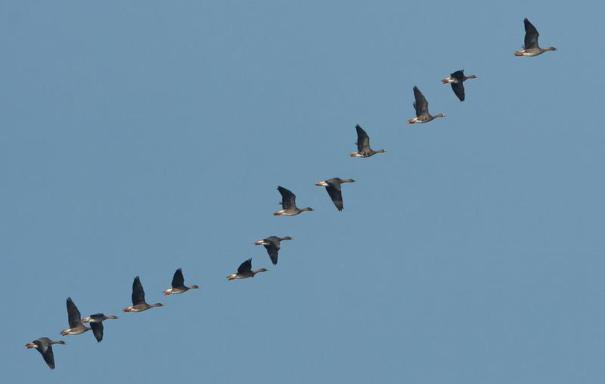
\includegraphics[height=0.19\linewidth,width=0.19\linewidth]{appendicies/raw_ims/541.jpg}%

\includegraphics[height=0.19\linewidth,width=0.19\linewidth]{appendicies/white.png}%
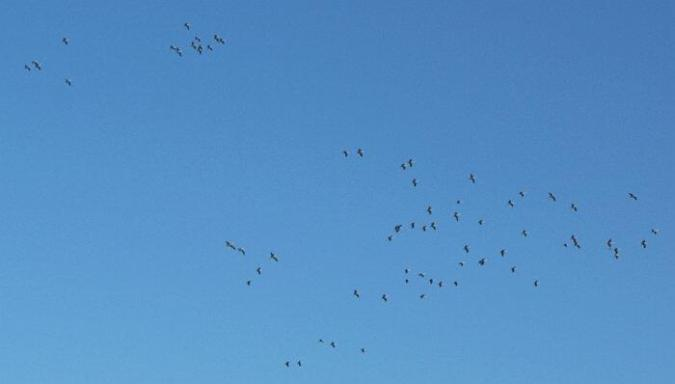
\includegraphics[height=0.19\linewidth,width=0.19\linewidth]{appendicies/raw_ims/4321.jpg}%
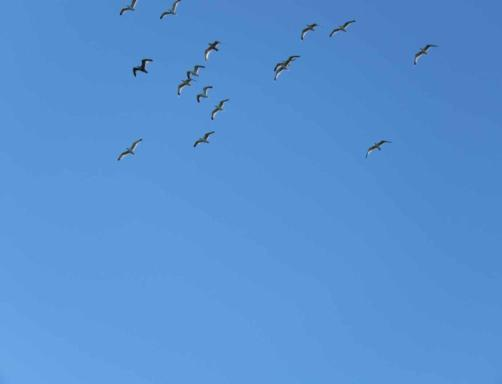
\includegraphics[height=0.19\linewidth,width=0.19\linewidth]{appendicies/raw_ims/4730.jpg}%
    \caption{Images that have a low pixel-wise difference that we deemed to be different.}
    \label{no_similar}
\end{figure*}
\begin{figure*}[!ht]
    \centering
    \fontsize{9}{9}\selectfont
    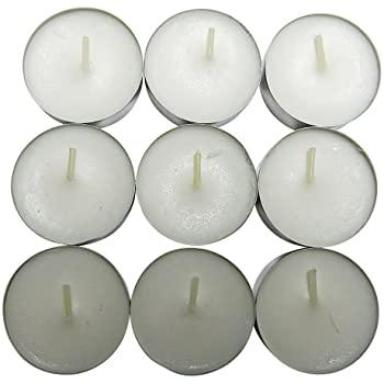
\includegraphics[height=0.19\linewidth, width=0.19\linewidth]{appendicies/raw_ims/3947.jpg}%
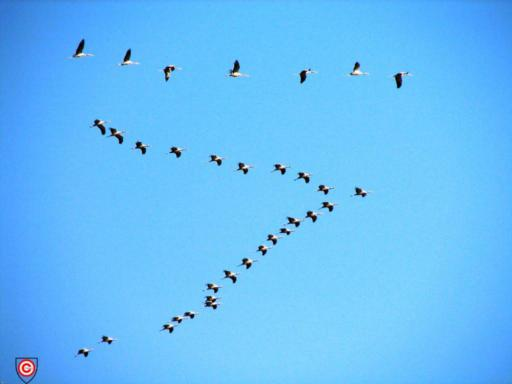
\includegraphics[height=0.19\linewidth, width=0.19\linewidth]{appendicies/raw_ims/4399.jpg}%

\includegraphics[height=0.19\linewidth, width=0.19\linewidth]{appendicies/raw_ims/3743.jpg}%
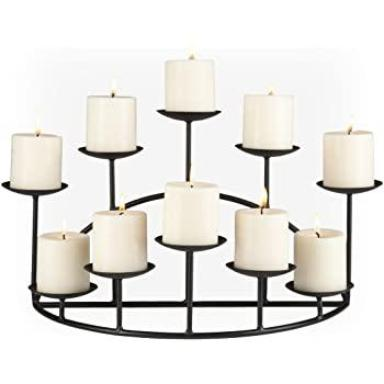
\includegraphics[height=0.19\linewidth, width=0.19\linewidth]{appendicies/raw_ims/3949.jpg}%

\includegraphics[height=0.19\linewidth, width=0.19\linewidth]{appendicies/raw_ims/5151.jpg}%
\\
\vspace{-0.0999em}
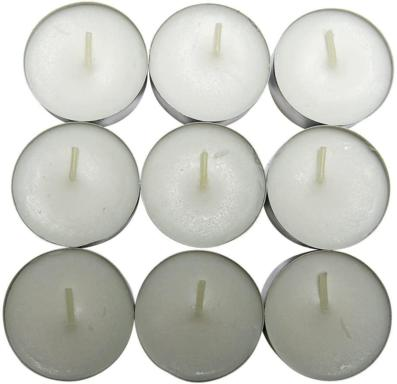
\includegraphics[height=0.19\linewidth, width=0.19\linewidth]{appendicies/raw_ims/5318.jpg}%
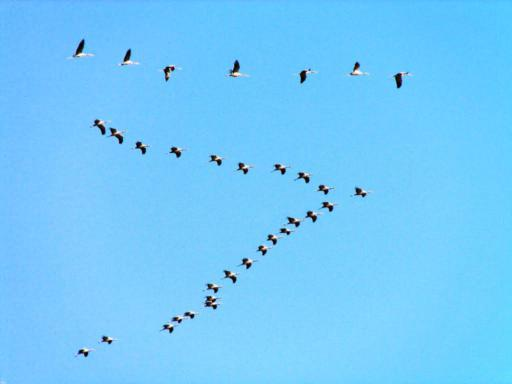
\includegraphics[height=0.19\linewidth, width=0.19\linewidth]{appendicies/raw_ims/4620.jpg}%
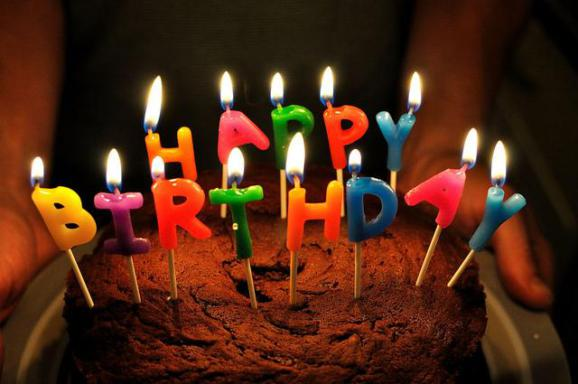
\includegraphics[height=0.19\linewidth, width=0.19\linewidth]{appendicies/raw_ims/5168.jpg}%
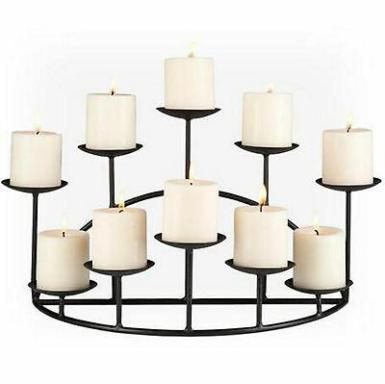
\includegraphics[height=0.19\linewidth, width=0.19\linewidth]{appendicies/raw_ims/3960.jpg}%

\includegraphics[height=0.19\linewidth, width=0.19\linewidth]{appendicies/raw_ims/5157.jpg}%
\\

    \caption{Examples of images at the upper bound of pixel-wise difference we considered that we deemed the same image. The pixel-wise differences of the images in each column when resized to 224$\times$224 are 5207, 5403, 7551, 8224 and 9396 respectively.}
    \label{similar}
\end{figure*}

\clearpage
\subsection{Similar Classes}\label{append_similar}
\begin{figure*}[!ht]    
    \centering
    \fontsize{8}{8}\selectfont
     Bread Rolls (Train)\\ \vspace{0.2em}
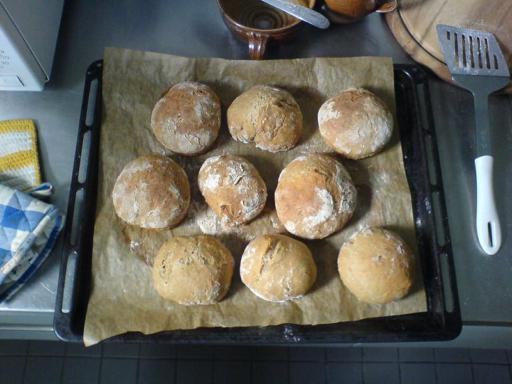
\includegraphics[height=0.09\textwidth,width=0.09\textwidth ]{appendicies/raw_ims/19.jpg}%
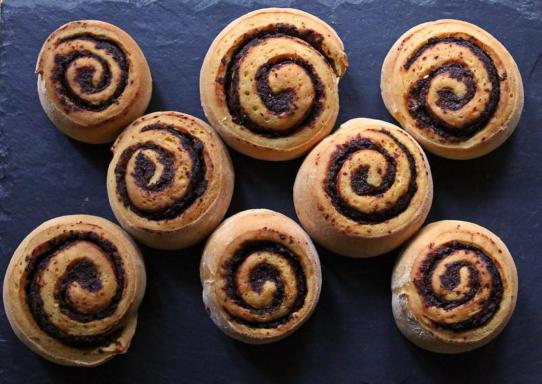
\includegraphics[height=0.09\textwidth,width=0.09\textwidth ]{appendicies/raw_ims/28.jpg}%
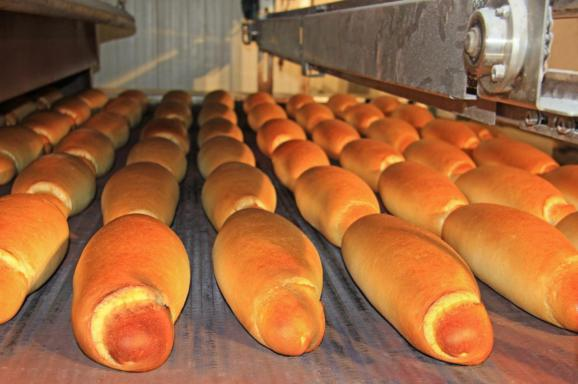
\includegraphics[height=0.09\textwidth,width=0.09\textwidth ]{appendicies/raw_ims/3381.jpg}%
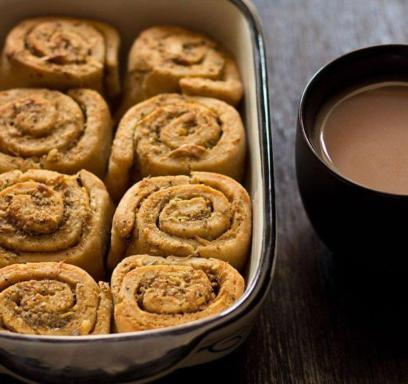
\includegraphics[height=0.09\textwidth,width=0.09\textwidth ]{appendicies/raw_ims/3394.jpg}%
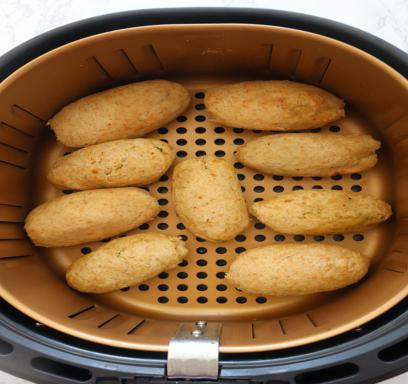
\includegraphics[height=0.09\textwidth,width=0.09\textwidth ]{appendicies/raw_ims/5966.jpg}%
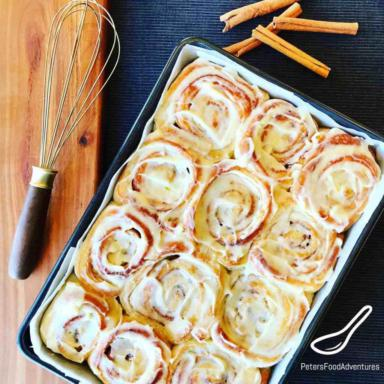
\includegraphics[height=0.09\textwidth,width=0.09\textwidth ]{appendicies/raw_ims/5974.jpg}%
\\ \vspace{0.2em}
 Buns (Train)\\
 \vspace{0.2em}
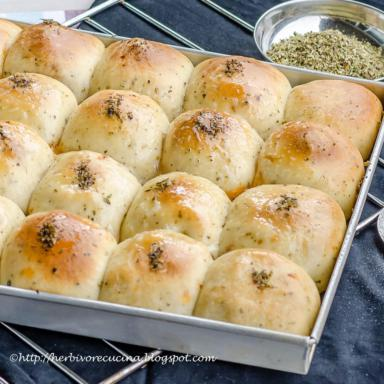
\includegraphics[height=0.09\textwidth,width=0.09\textwidth ]{appendicies/raw_ims/3676.jpg}%
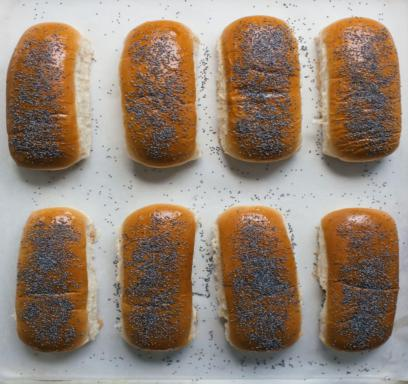
\includegraphics[height=0.09\textwidth,width=0.09\textwidth ]{appendicies/raw_ims/3681.jpg}%
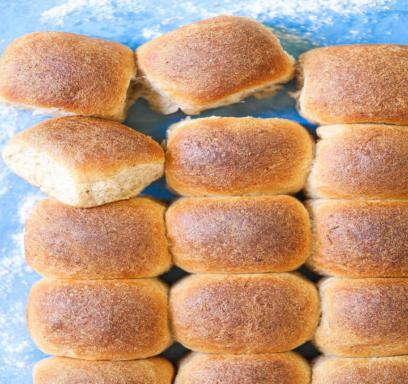
\includegraphics[height=0.09\textwidth,width=0.09\textwidth ]{appendicies/raw_ims/3684.jpg}%
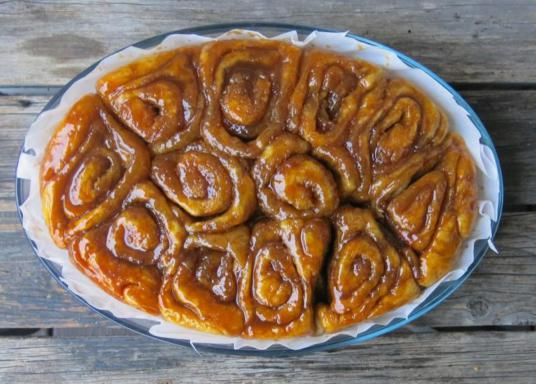
\includegraphics[height=0.09\textwidth,width=0.09\textwidth ]{appendicies/raw_ims/3685.jpg}%
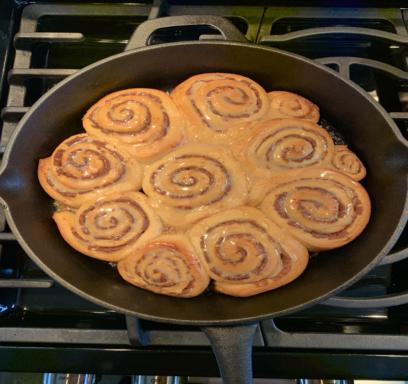
\includegraphics[height=0.09\textwidth,width=0.09\textwidth ]{appendicies/raw_ims/3691.jpg}%
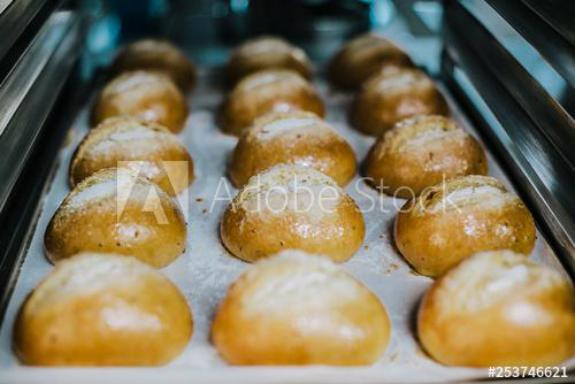
\includegraphics[height=0.09\textwidth,width=0.09\textwidth ]{appendicies/raw_ims/3680.jpg}%
\\ \vspace{0.2em}
 Baguette Rolls (Train)\\ \vspace{0.2em}
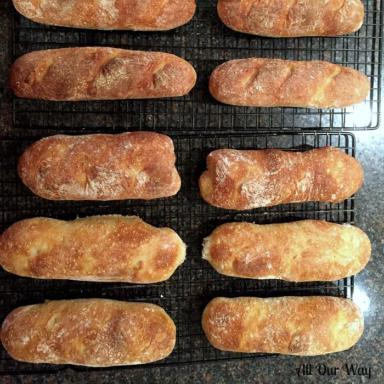
\includegraphics[height=0.09\textwidth,width=0.09\textwidth ]{appendicies/raw_ims/3511.jpg}%
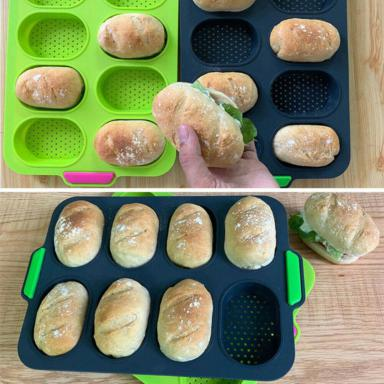
\includegraphics[height=0.09\textwidth,width=0.09\textwidth ]{appendicies/raw_ims/3512.jpg}%
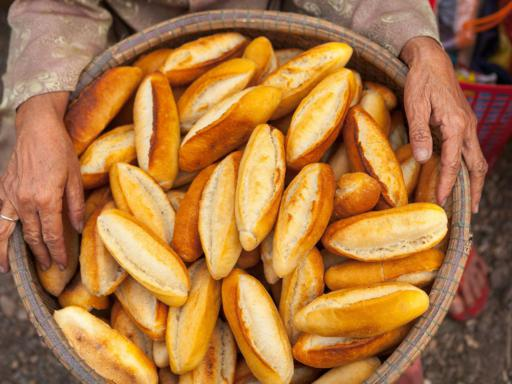
\includegraphics[height=0.09\textwidth,width=0.09\textwidth ]{appendicies/raw_ims/3514.jpg}%
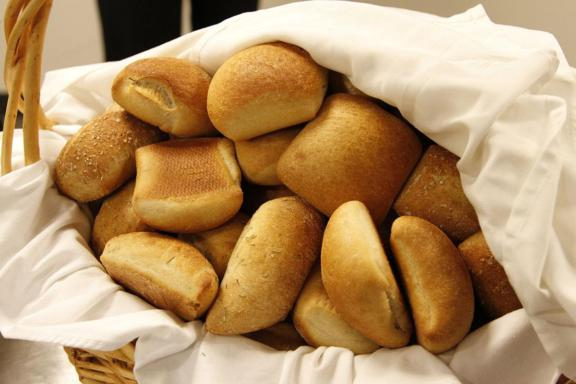
\includegraphics[height=0.09\textwidth,width=0.09\textwidth ]{appendicies/raw_ims/3515.jpg}%
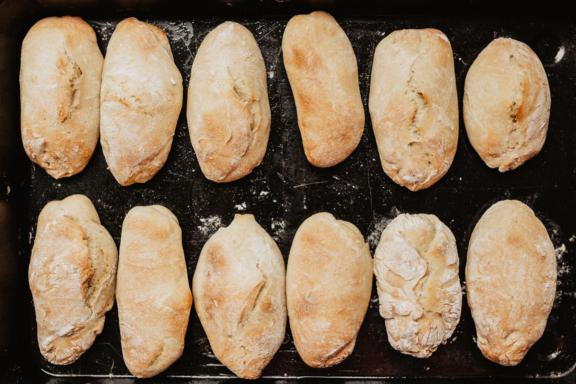
\includegraphics[height=0.09\textwidth,width=0.09\textwidth ]{appendicies/raw_ims/3516.jpg}%

\includegraphics[height=0.09\textwidth,width=0.09\textwidth ]{appendicies/white.png}%
\\  \vspace{0.2em}
 Red Beans (Test)\\  \vspace{0.2em}
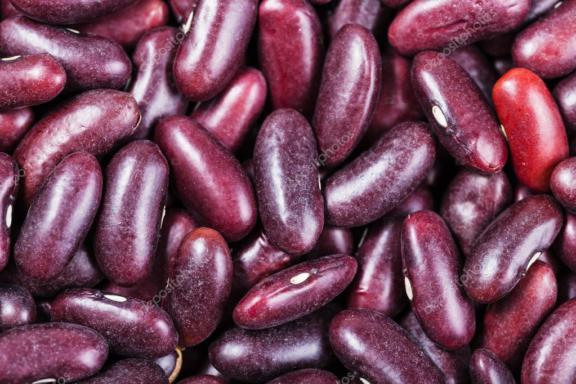
\includegraphics[height=0.09\textwidth,width=0.09\textwidth ]{appendicies/raw_ims/3493.jpg}%
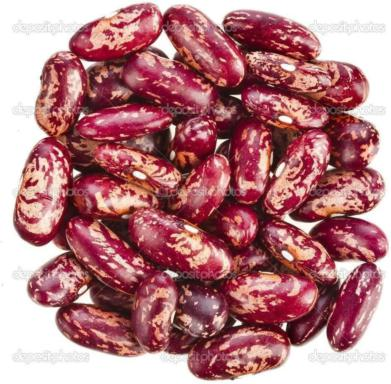
\includegraphics[height=0.09\textwidth,width=0.09\textwidth ]{appendicies/raw_ims/3494.jpg}%
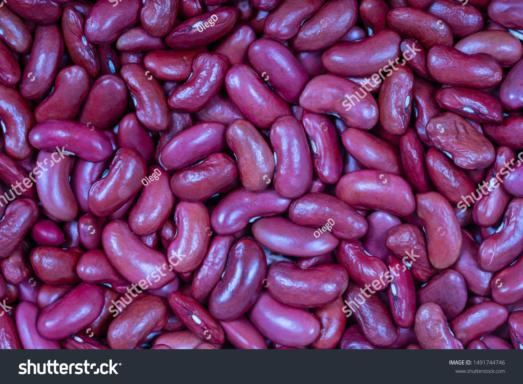
\includegraphics[height=0.09\textwidth,width=0.09\textwidth ]{appendicies/raw_ims/3495.jpg}%
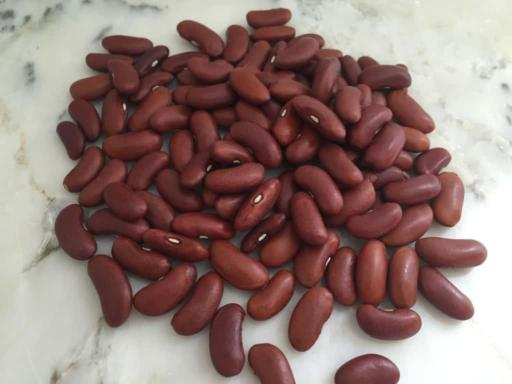
\includegraphics[height=0.09\textwidth,width=0.09\textwidth ]{appendicies/raw_ims/3498.jpg}%
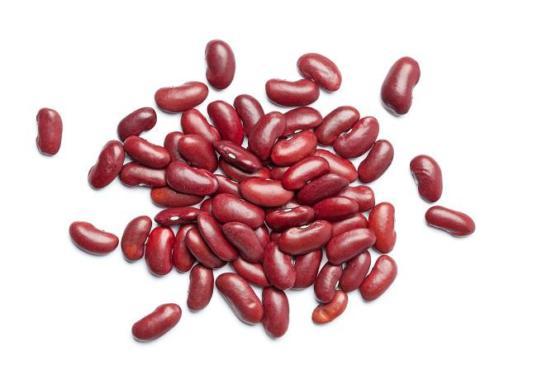
\includegraphics[height=0.09\textwidth,width=0.09\textwidth ]{appendicies/raw_ims/3501.jpg}%
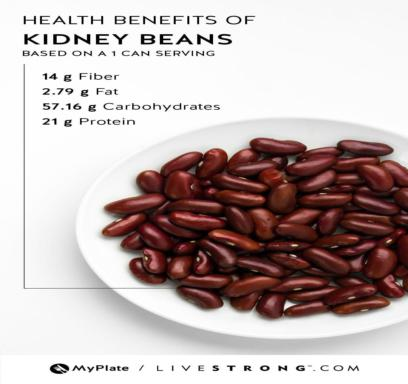
\includegraphics[height=0.09\textwidth,width=0.09\textwidth ]{appendicies/raw_ims/3502.jpg}%
\\  \vspace{0.2em}
 Kidney Beans (Train)\\  \vspace{0.2em}
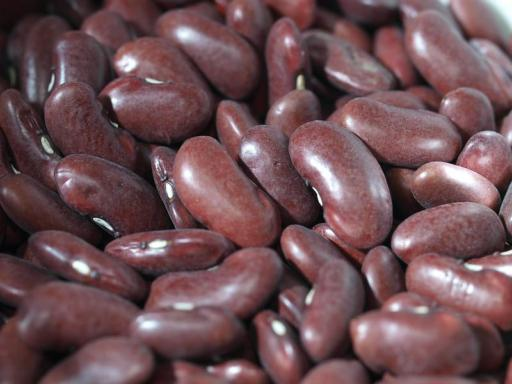
\includegraphics[height=0.09\textwidth,width=0.09\textwidth ]{appendicies/raw_ims/3224.jpg}%
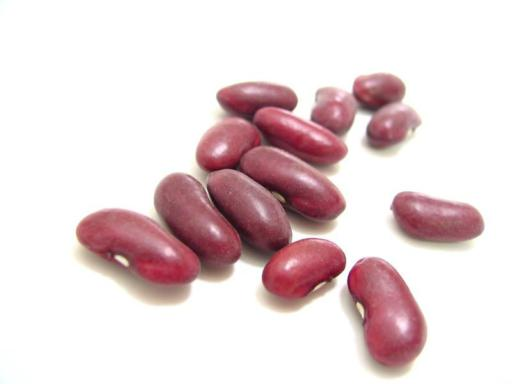
\includegraphics[height=0.09\textwidth,width=0.09\textwidth ]{appendicies/raw_ims/3227.jpg}%
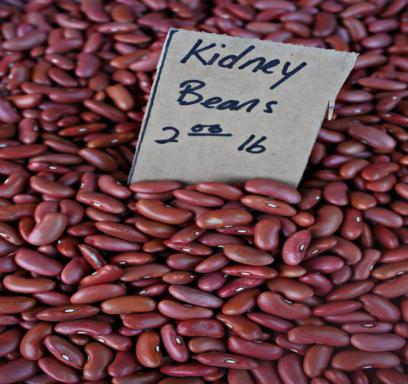
\includegraphics[height=0.09\textwidth,width=0.09\textwidth ]{appendicies/raw_ims/3231.jpg}%
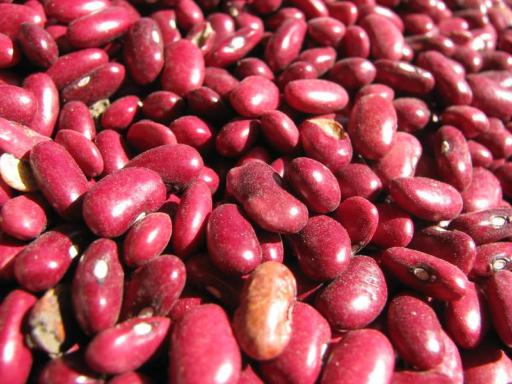
\includegraphics[height=0.09\textwidth,width=0.09\textwidth ]{appendicies/raw_ims/3233.jpg}%
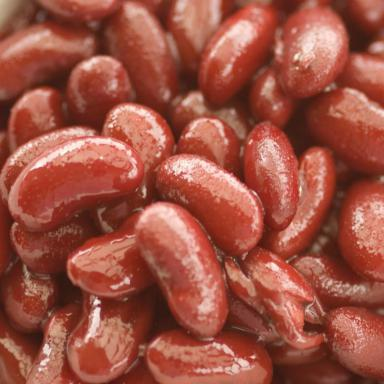
\includegraphics[height=0.09\textwidth,width=0.09\textwidth ]{appendicies/raw_ims/3234.jpg}%
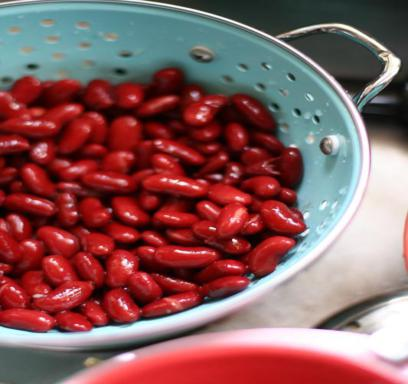
\includegraphics[height=0.09\textwidth,width=0.09\textwidth ]{appendicies/raw_ims/3235.jpg}% 
\\  \vspace{0.2em}
 Birds (Val)\\  \vspace{0.2em}
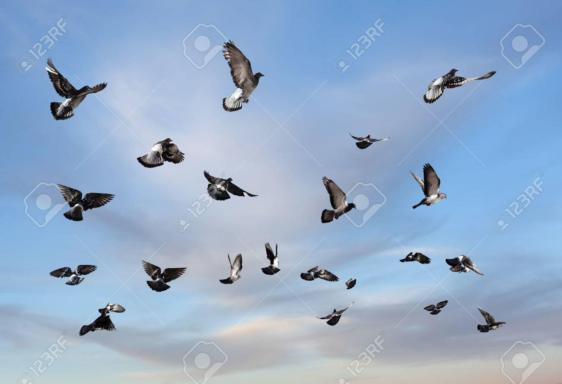
\includegraphics[height=0.09\textwidth,width=0.09\textwidth ]{appendicies/raw_ims/929.jpg}%
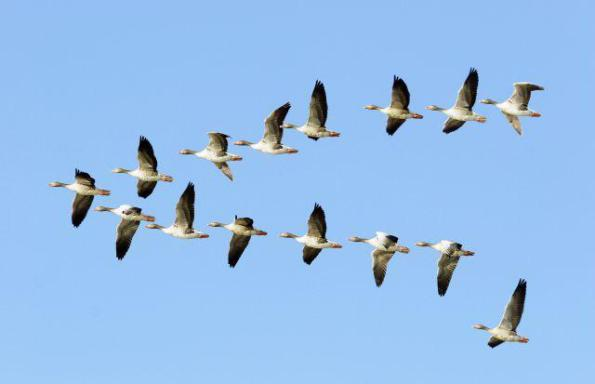
\includegraphics[height=0.09\textwidth,width=0.09\textwidth ]{appendicies/raw_ims/930.jpg}%
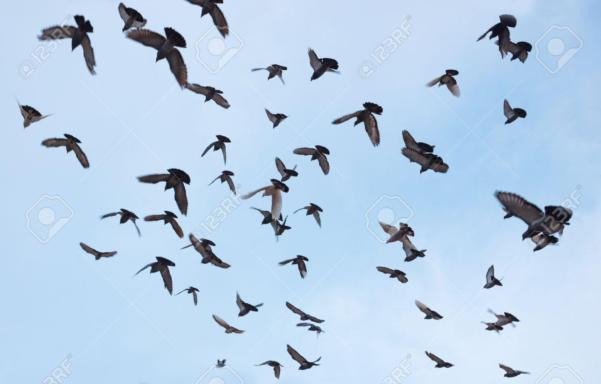
\includegraphics[height=0.09\textwidth,width=0.09\textwidth ]{appendicies/raw_ims/932.jpg}%
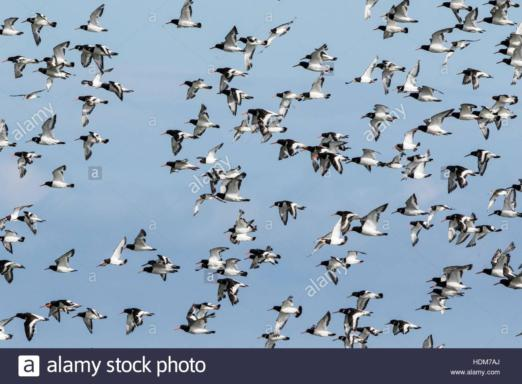
\includegraphics[height=0.09\textwidth,width=0.09\textwidth ]{appendicies/raw_ims/945.jpg}%
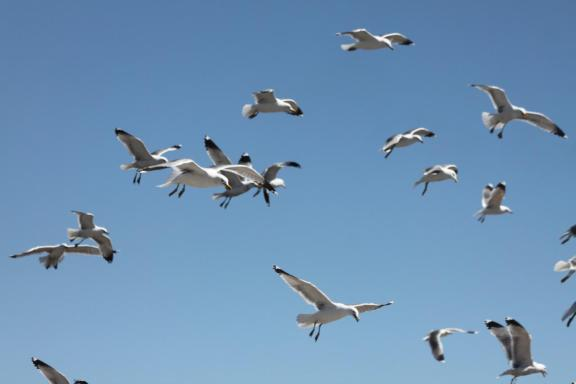
\includegraphics[height=0.09\textwidth,width=0.09\textwidth ]{appendicies/raw_ims/959.jpg}%
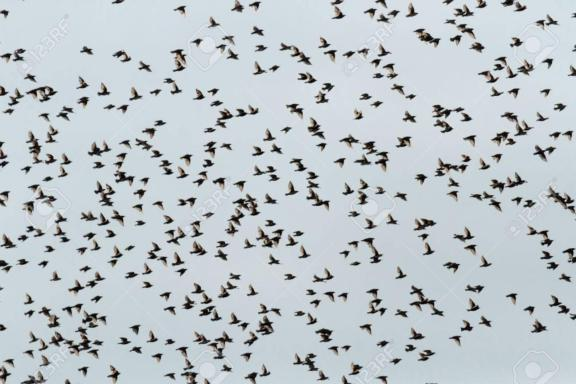
\includegraphics[height=0.09\textwidth,width=0.09\textwidth ]{appendicies/raw_ims/972.jpg}% 
\\  \vspace{0.2em}
 Cranes (Train)\\  \vspace{0.2em}
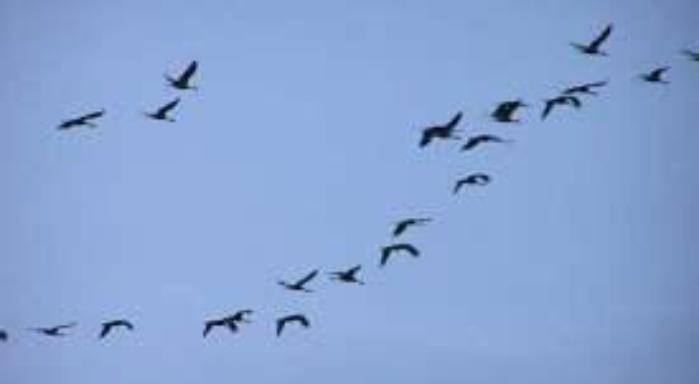
\includegraphics[height=0.09\textwidth,width=0.09\textwidth ]{appendicies/raw_ims/5953.jpg}%
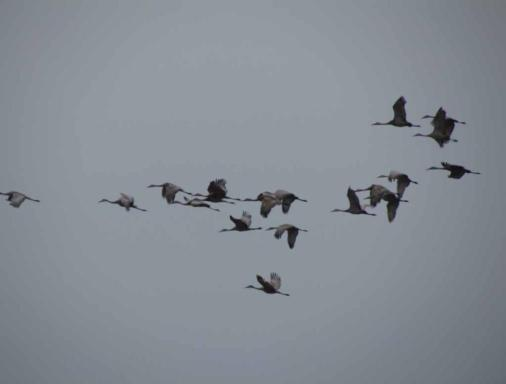
\includegraphics[height=0.09\textwidth,width=0.09\textwidth ]{appendicies/raw_ims/5954.jpg}%
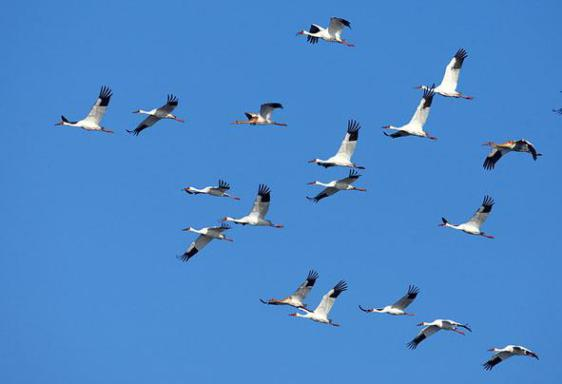
\includegraphics[height=0.09\textwidth,width=0.09\textwidth ]{appendicies/raw_ims/5956.jpg}%
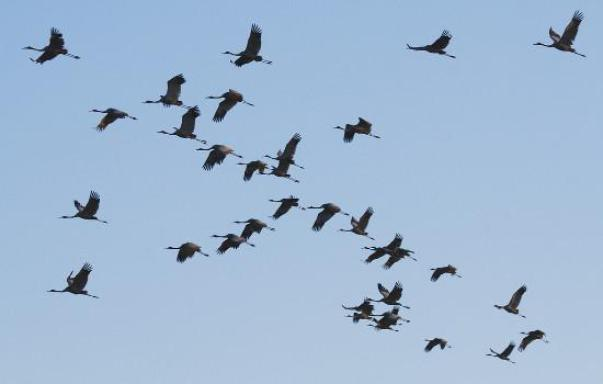
\includegraphics[height=0.09\textwidth,width=0.09\textwidth ]{appendicies/raw_ims/5957.jpg}%
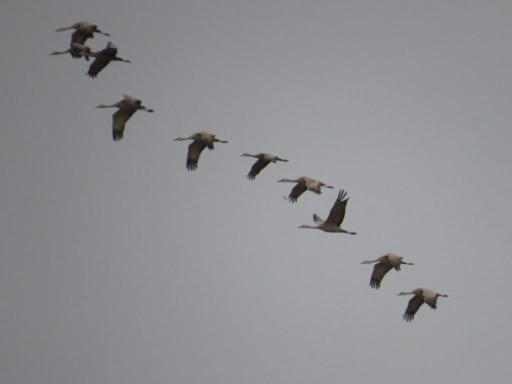
\includegraphics[height=0.09\textwidth,width=0.09\textwidth ]{appendicies/raw_ims/5959.jpg}%
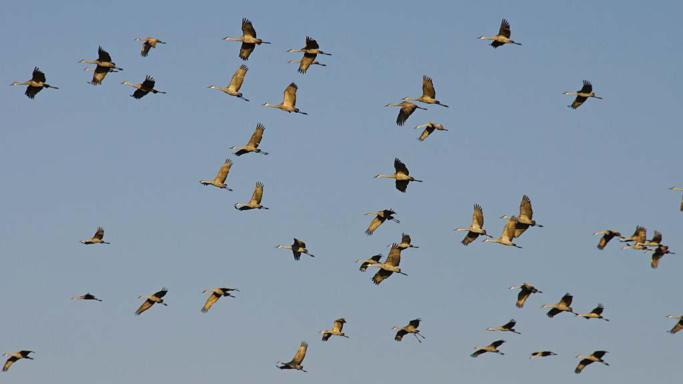
\includegraphics[height=0.09\textwidth,width=0.09\textwidth ]{appendicies/raw_ims/5960.jpg}% 
\\  \vspace{0.2em}
 Flamingos (Val)\\  \vspace{0.2em}
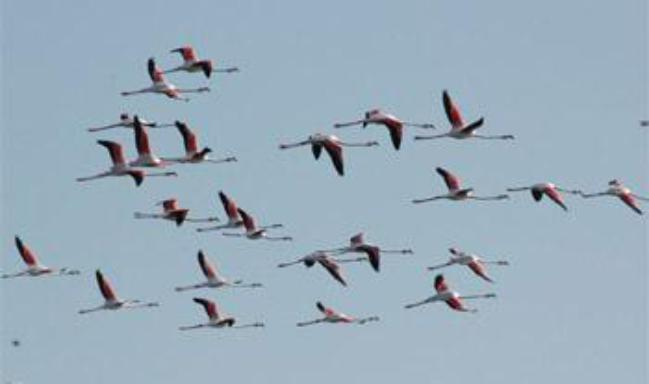
\includegraphics[height=0.09\textwidth,width=0.09\textwidth ]{appendicies/raw_ims/6070.jpg}%
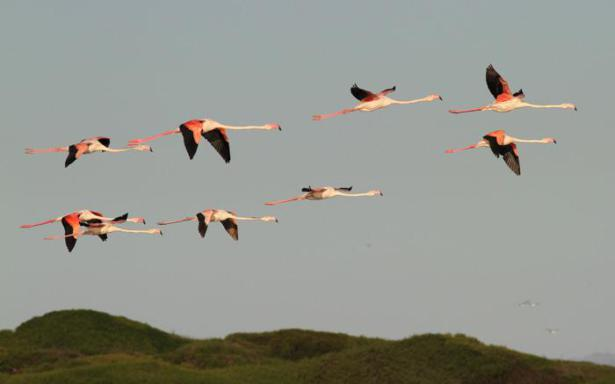
\includegraphics[height=0.09\textwidth,width=0.09\textwidth ]{appendicies/raw_ims/6071.jpg}%
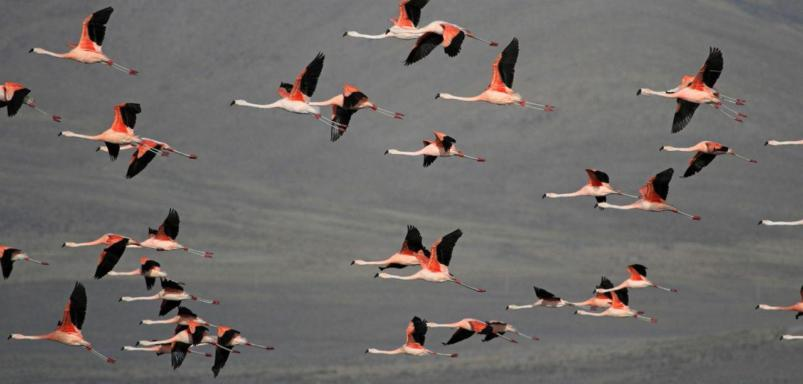
\includegraphics[height=0.09\textwidth,width=0.09\textwidth ]{appendicies/raw_ims/6072.jpg}%
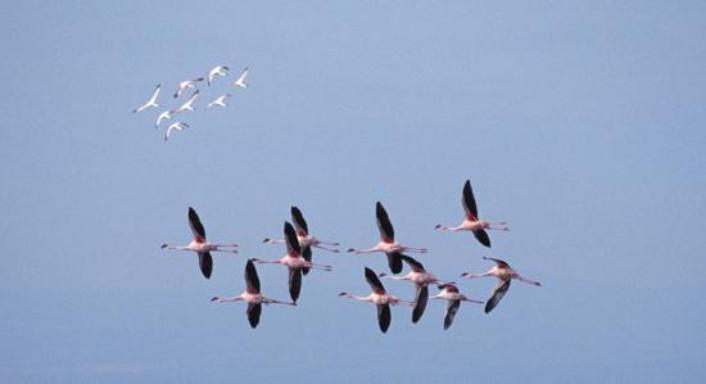
\includegraphics[height=0.09\textwidth,width=0.09\textwidth ]{appendicies/raw_ims/6073.jpg}%
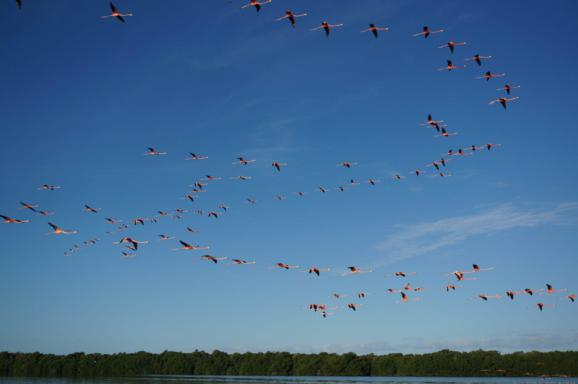
\includegraphics[height=0.09\textwidth,width=0.09\textwidth ]{appendicies/raw_ims/6075.jpg}%
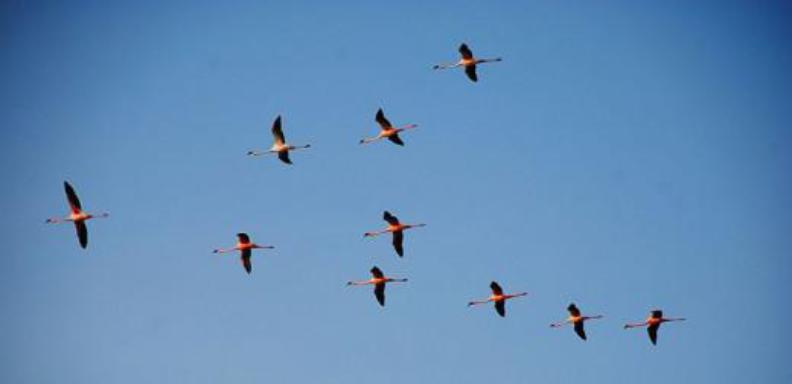
\includegraphics[height=0.09\textwidth,width=0.09\textwidth ]{appendicies/raw_ims/6079.jpg}% 
\\  \vspace{0.2em}
 Geese (Train)\\  \vspace{0.2em}
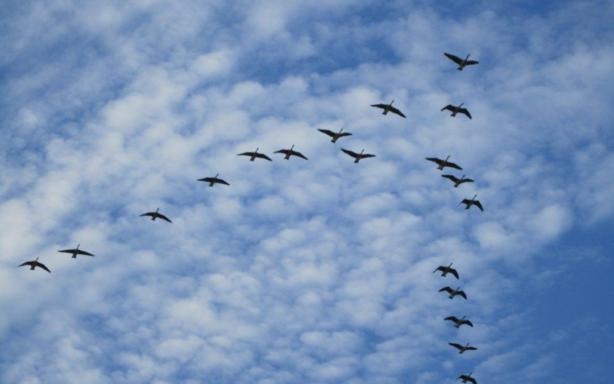
\includegraphics[height=0.09\textwidth,width=0.09\textwidth ]{appendicies/raw_ims/4612.jpg}%
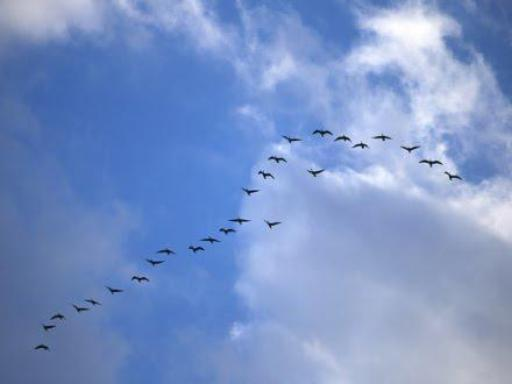
\includegraphics[height=0.09\textwidth,width=0.09\textwidth ]{appendicies/raw_ims/4613.jpg}%
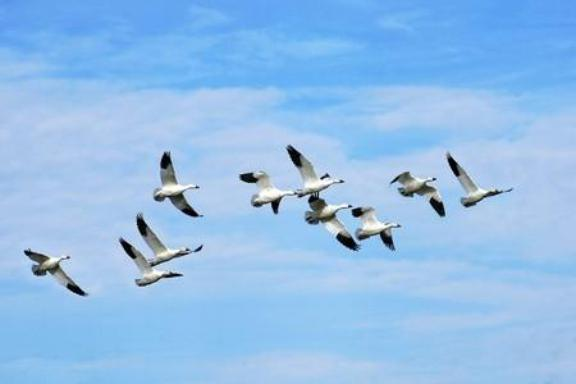
\includegraphics[height=0.09\textwidth,width=0.09\textwidth ]{appendicies/raw_ims/4615.jpg}%
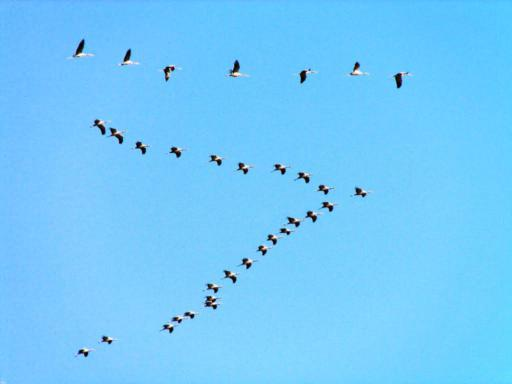
\includegraphics[height=0.09\textwidth,width=0.09\textwidth ]{appendicies/raw_ims/4620.jpg}%
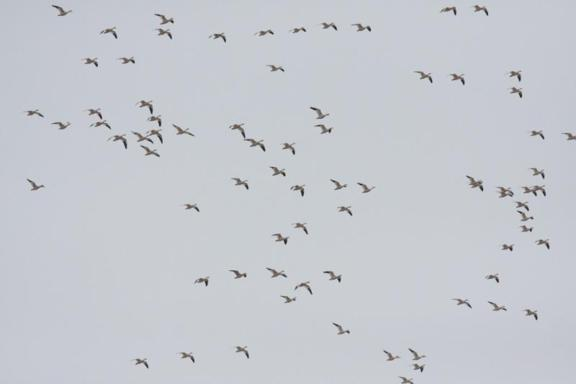
\includegraphics[height=0.09\textwidth,width=0.09\textwidth ]{appendicies/raw_ims/4627.jpg}%
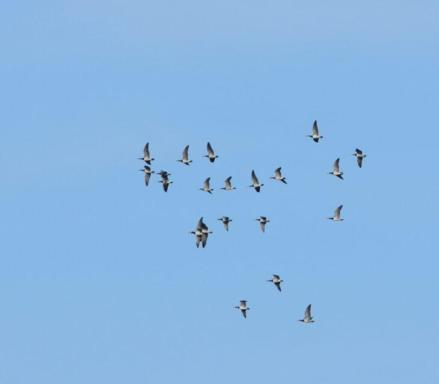
\includegraphics[height=0.09\textwidth,width=0.09\textwidth ]{appendicies/raw_ims/4628.jpg}% 
\\  \vspace{0.2em}
 Seagulls (Val)\\  \vspace{0.2em}
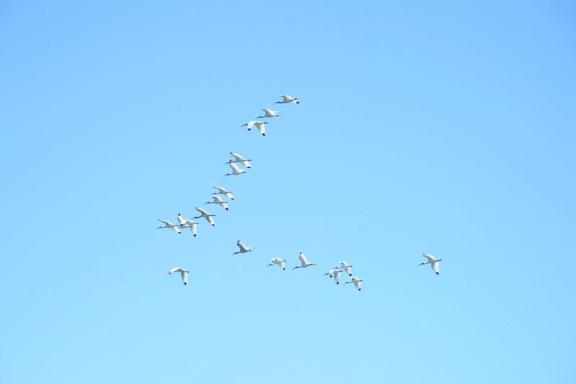
\includegraphics[height=0.09\textwidth,width=0.09\textwidth ]{appendicies/raw_ims/192.jpg}%
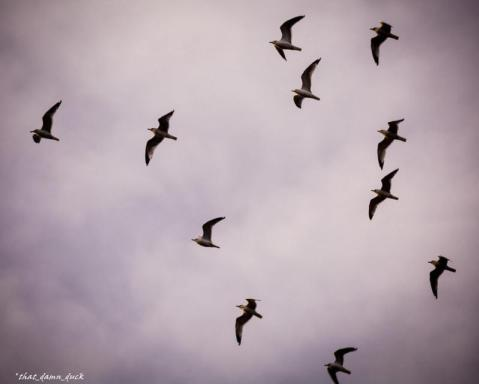
\includegraphics[height=0.09\textwidth,width=0.09\textwidth ]{appendicies/raw_ims/591.jpg}%
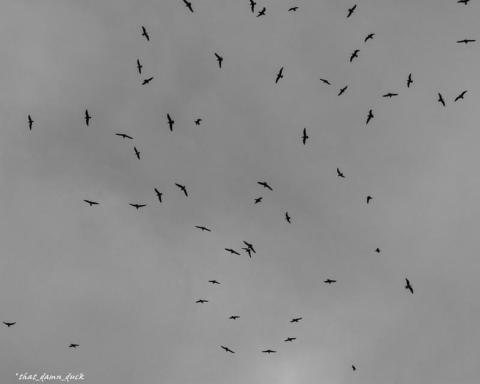
\includegraphics[height=0.09\textwidth,width=0.09\textwidth ]{appendicies/raw_ims/597.jpg}%
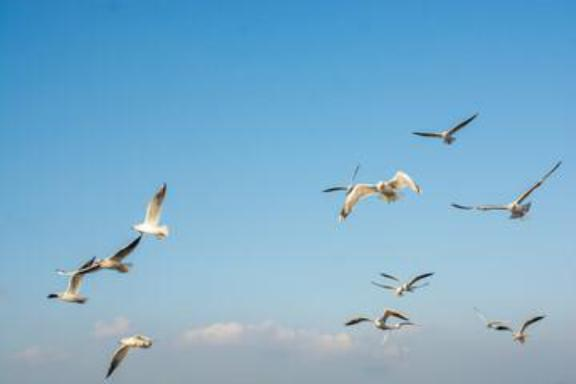
\includegraphics[height=0.09\textwidth,width=0.09\textwidth ]{appendicies/raw_ims/4703.jpg}%
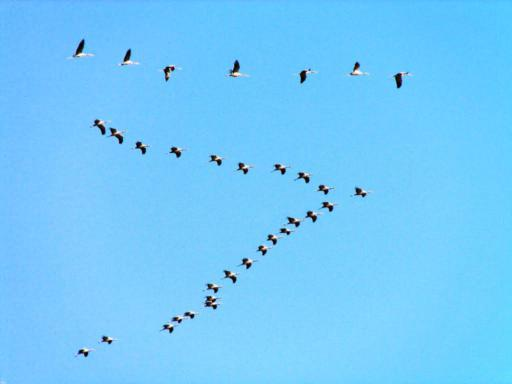
\includegraphics[height=0.09\textwidth,width=0.09\textwidth ]{appendicies/raw_ims/4719.jpg}%
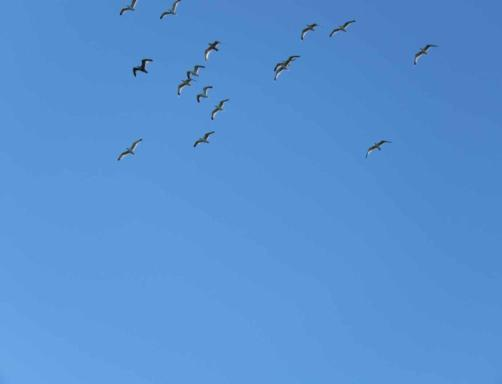
\includegraphics[height=0.09\textwidth,width=0.09\textwidth ]{appendicies/raw_ims/4730.jpg}%
\\
    \caption{Examples of clear overlap or similarity between classes. Each row has a different class label in FSC-147. In FSC-133 these are simplified to Bread Rolls (Train), Kidney Beans (Train) and Birds (Train).}
    \label{arethesame}
\end{figure*}


\clearpage

% \subsection{Annotation Errors}\label{append_annotation_errors}
% \begin{figure*}[!ht]    
%     \centering
%     \fontsize{8}{8}\selectfont
%     \input{appendicies/annotation_errors}
%     \caption{Examples of errors in the FSC-147 annotations. Rows 1 \& 3 show the image and the bounding box annotations, rows 2 \& 4 show the image, the bounding box annotations and the ground truth density map generated from the instance dot annotations.}
%     \label{Fig_annotation_errors}
% \end{figure*}


\clearpage

\subsection{Duplicate Discrepancies}\label{discrepancies}
\begin{table*}[!ht]
    \centering
    \fontsize{9}{9}\selectfont
    \resizebox*{0.42\textheight}{!}{
        \begin{tabular}{clrlclrlrlc}
 \toprule
\multicolumn{4}{c}{Image A} & \multicolumn{4}{c}{Image B} & \multicolumn{2}{c}{Count Diff} \\
ID & Class & Count & Set & Id & Class & Count & Set & Abs & Rel & Kept\\
\cmidrule(r){1-4} \cmidrule(r){5-8} \cmidrule(r){9-10} \cmidrule(r){11-11}

4399 & cranes & 26 & train & 4549 & flamingos & 33 & val & 7 & 0.21 & A\\
4399 & cranes & 26 & train & 4719 & seagulls & 33 & val & 7 & 0.21 & A \\
2891 & caps & 144 & train & 1896 & bottle caps & 123 & val & 21 & 0.15 & B \\
4386 & cranes & 20 & train & 7415 & birds & 23 & val & 3 & 0.13 & A\\
6567 & pigeons & 21 & train & 929 & birds & 23 & val & 2 & 0.09 & A\\
4664 & geese & 11 & train & 6873 & birds & 11 & val & 0 & 0.00 & A\\
4613 & geese & 26 & train & 6714 & birds & 26 & val & 0 & 0.00 & B\\
4350 & cranes & 8 & train & 4704 & seagulls & 8 & val & 0 & 0.00 & 4683 \\
4350 & cranes & 8 & train & 4707 & seagulls & 8 & val & 0 & 0.00 & 4683\\
3506 & m\&m pieces & 111 & train & 3698 & candy pieces & 111 & test & 0 & 0.00 & A\\
3791 & kidney beans & 37 & train & 3494 & red beans & 37 & test & 0 & 0.00 & A\\

\bottomrule
\end{tabular}}
        \caption{The 17 cases where the same image appears in more than on of the: train set, validation or test set. The right column denotes which of these images, or if a third images appears in FSC-133.}
    \label{FSC_SPLIT_LEAK}
\end{table*}

\begin{table*}[!ht]
    \centering
    \fontsize{9}{9}\selectfont
       % \resizebox{0.6\textwidth}{!}{
    \resizebox*{0.42\textheight}{!}{
    \begin{tabular}{clrlclrlrlc}
 \toprule
\multicolumn{4}{c}{Image A} & \multicolumn{4}{c}{Image B} & \multicolumn{2}{c}{Count Diff} \\
ID & Class & Count & Set & Id & Class & Count & Set & Abs & Rel & Kept\\
\cmidrule(r){1-4} \cmidrule(r){5-8} \cmidrule(r){9-10} \cmidrule(r){11-11} 
5223 & donuts tray & 9 & val & 5664 & donuts tray & 12 & val & 3 & 0.25 & A\\
613 & seagulls & 7 & val & 623 & seagulls & 9 & val & 2 & 0.22 & B\\
4399 & cranes & 26 & train & 4549 & flamingos & 33 & val & 7 & 0.21 & 4683\\
4399 & cranes & 26 & train & 4620 & geese & 33 & train & 7 & 0.21 & 4683\\
4399 & cranes & 26 & train & 4719 & seagulls & 33 & val & 7 & 0.21 & 4683\\
3812 & cupcakes & 10 & train & 5238 & cupcakes & 8 & train & 2 & 0.20 & B \\
5142 & cashew nuts & 193 & test & 5801 & cashew nuts & 157 & test & 36 & 0.19 & B\\
4634 & geese & 18 & train & 6143 & geese & 15 & train & 3 & 0.17 & A\\
4634 & geese & 18 & train & 6669 & geese & 15 & train & 3 & 0.17 & A \\
6850 & cereals & 25 & train & 7337 & cereals & 21 & train & 4 & 0.16 & B\\
6839 & watches & 58 & test & 989 & watches & 69 & test & 11 & 0.16 & A\\
1896 & bottle caps & 123 & val & 2891 & caps & 144 & train & 21 & 0.15 & A\\
2717 & oranges & 94 & train & 6573 & oranges & 110 & train & 16 & 0.15 & A\\
3648 & cashew nuts & 35 & test & 5141 & cashew nuts & 30 & test & 5 & 0.14 & B\\
3014 & mini blinds & 26 & train & 7307 & mini blinds & 30 & train & 4 & 0.13 & A \\
4386 & cranes & 20 & train & 7415 & birds & 23 & val & 3 & 0.13 & A\\
2970 & fishes & 16 & train & 6953 & fishes & 18 & train & 2 & 0.11 & B\\
5929 & eggs & 76 & test & 6852 & eggs & 68 & test & 8 & 0.11 & B\\
4295 & green peas & 110 & test & 5504 & green peas & 122 & test & 12 & 0.10 & A\\
6567 & pigeons & 21 & train & 929 & birds & 23 & val & 2 & 0.09 & A\\
2743 & oranges & 57 & train & 7363 & oranges & 52 & train & 5 & 0.09 & B\\
6138 & cars & 122 & train & 6864 & cars & 111 & train & 11 & 0.09 & A\\
4220 & biscuits & 11 & train & 5422 & biscuits & 10 & train & 1 & 0.09 & B\\
3282 & finger foods & 31 & test & 3285 & finger foods & 34 & test & 3 & 0.09 & A\\
3462 & beads & 92 & train & 5638 & beads & 85 & train & 7 & 0.08 & A\\
4040 & beads & 117 & train & 5760 & beads & 108 & train & 9 & 0.08 & A\\
3492 & polka dots & 25 & val & 5738 & polka dots & 27 & val & 2 & 0.07 & A\\
3486 & polka dots & 81 & val & 5740 & polka dots & 87 & val & 6 & 0.07 & A\\
6917 & cereals & 29 & train & 7353 & cereals & 27 & train & 2 & 0.07 & B\\
5209 & donuts tray & 17 & val & 5656 & donuts tray & 16 & val & 1 & 0.06 & B\\
4013 & beads & 115 & train & 5754 & beads & 108 & train & 7 & 0.06 & B\\
524 & geese & 30 & train & 635 & cranes & 32 & train & 2 & 0.06 & B\\
4300 & green peas & 83 & test & 5506 & green peas & 88 & test & 5 & 0.06 & A\\
3287 & macarons & 16 & train & 428 & macarons & 17 & train & 1 & 0.06 & A \\
4634 & geese & 18 & train & 4675 & geese & 17 & train & 1 & 0.06 & A\\
6602 & pencils & 38 & train & 7400 & pencils & 36 & train & 2 & 0.05 & B \\
3475 & beads & 108 & train & 5637 & beads & 103 & train & 5 & 0.05 & A\\
2357 & bricks & 276 & train & 2401 & bricks & 263 & train & 13 & 0.05 & B\\
4044 & beads & 115 & train & 5335 & beads & 109 & train & 6 & 0.05 & A\\
4019 & beads & 105 & train & 5771 & beads & 109 & train & 4 & 0.04 & A\\
4049 & beads & 26 & train & 5755 & beads & 27 & train & 1 & 0.04 & B\\
3956 & candles & 46 & train & 5309 & candles & 44 & train & 2 & 0.04 & B \\
3969 & candles & 23 & train & 5317 & candles & 24 & train & 1 & 0.04 & A \\
3950 & candles & 24 & train & 5312 & candles & 25 & train & 1 & 0.04 & A\\
3020 & mini blinds & 34 & train & 7630 & mini blinds & 35 & train & 1 & 0.03 & A\\
3668 & toilet paper rolls & 31 & val & 5154 & toilet paper rolls & 32 & val & 1 & 0.03 & A\\
3679 & buns & 35 & train & 5026 & bread rolls & 36 & train & 1 & 0.03 & A\\
4014 & beads & 108 & train & 5749 & beads & 105 & train & 3 & 0.03 & A\\
3645 & cashew nuts & 60 & test & 5797 & cashew nuts & 58 & test & 2 & 0.03 & A\\
5148 & cashew nuts & 36 & test & 5803 & cashew nuts & 35 & test & 1 & 0.03 & A\\
7640 & apples & 32 & test & 7665 & apples & 33 & test & 1 & 0.03 & B\\
3819 & cupcakes & 36 & train & 5241 & cupcakes & 35 & train & 1 & 0.03 & B\\
3754 & pearls & 131 & train & 5185 & pearls & 127 & train & 4 & 0.03 & B\\
3666 & toilet paper rolls & 32 & val & 5157 & toilet paper rolls & 31 & val & 1 & 0.03 & B\\
3639 & jade stones & 31 & train & 5134 & jade stones & 32 & train & 1 & 0.03 & A\\
6200 & coins & 52 & train & 6228 & coins & 53 & train & 1 & 0.02 & A\\
267 & beads & 59 & train & 3242 & beads & 60 & train & 1 & 0.02 & A\\
6798 & birds & 87 & val & 976 & birds & 85 & val & 2 & 0.02 & B\\
3795 & kidney beans & 53 & train & 5547 & kidney beans & 52 & train & 1 & 0.02 & B\\
3955 & candles & 60 & train & 5306 & candles & 61 & train & 1 & 0.02 & A\\
2671 & bowls & 60 & train & 6724 & bowls & 59 & train & 1 & 0.02 & B\\
6738 & mini blinds & 53 & train & 7130 & mini blinds & 52 & train & 1 & 0.02 & B\\
5053 & beads & 139 & train & 5644 & beads & 136 & train & 3 & 0.02 & B\\
3426 & polka dots & 219 & val & 5046 & polka dots & 215 & val & 4 & 0.02 & B\\
3122 & coffee beans & 90 & train & 3134 & coffee beans & 89 & train & 1 & 0.01 & B\\
6961 & cartridges & 178 & train & 7680 & cartridges & 179 & train & 1 & 0.01 & A\\
4016 & beads & 109 & train & 5333 & beads & 108 & train & 1 & 0.01 & B\\
3469 & beads & 74 & train & 5050 & beads & 75 & train & 1 & 0.01 & A\\
4021 & beads & 106 & train & 5759 & beads & 107 & train & 1 & 0.01 & B\\
5149 & cashew nuts & 111 & test & 5807 & cashew nuts & 110 & test & 1 & 0.01 & B\\
4044 & beads & 115 & train & 5767 & beads & 116 & train & 1 & 0.01 & A\\
\bottomrule
\end{tabular}
}
     \caption{The 71 cases where the same image appears more than once in FSC-147 with different associated counts. The right column denotes which of these images, or if a third images appears in FSC-133.}
    \label{FSC_COUNT_DIFF}
    
\end{table*}
\clearpage

\subsection{FSC-147 and FSC-133 Class Split}\label{append_classes}
\begin{table*}[!ht]
    \centering
    \fontsize{9}{9}\selectfont
    \begin{tabular}{ccccc}
 \toprule

\multicolumn{5}{c}{Train} \\
\midrule
\textbf{alcohol bottles}&\textbf{baguette rolls}&balls&bananas&beads\\
bees&birthday candles&biscuits&boats&bottles\\
bowls&boxes&bread rolls&bricks&buffaloes\\
\textbf{buns}&calamari rings&candles&cans&caps\\
cars&cartridges&cassettes&cement bags&cereals\\
chewing gum pieces&chopstick&clams&coffee beans&coins\\
cotton balls&cows&\textbf{cranes}&crayons&croissants\\
\textbf{crows}&cupcake tray&cupcakes&cups&fishes\\
\textbf{geese}&gemstones&go game&goats&goldfish snack\\
ice cream&instant noodles&jade stones&jeans&kidney beans\\
kitchen towels&lighters&lipstick&m\&m pieces&macarons\\
matches&meat skewers&mini blinds&mosaic tiles&naan bread\\
nails&nuts&onion rings&oranges&pearls\\
pencils&penguins&pens&people&peppers\\
\textbf{pigeons}&plates&polka dot tiles&potatoes&rice bags\\
roof tiles&screws&shoes&spoon&spring rolls\\
stairs&stapler pins&straws&supermarket shelf&\textbf{swans}\\
tomatoes&watermelon&windows&zebras\\

\midrule
\multicolumn{5}{c}{Val} \\
\midrule
ants&\textcolor{blue}{birds}&books&bottle caps&bullets\\
camels&chairs&chicken wings&donuts tray&\textbf{\textcolor{blue}{flamingos}}\\
flower pots&flowers&fresh cut&grapes&horses\\
kiwis&milk cartons&oyster shells&oysters&peaches\\
pills&polka dots&prawn crackers&sausages&\textbf{\textcolor{blue}{seagulls}}\\
shallots&shirts&skateboard&toilet paper rolls\\

\midrule
\multicolumn{5}{c}{Test} \\
\midrule
apples&candy pieces&carrom board pieces&\textbf{\textcolor{blue}{cashew nuts}}&comic books\\
crab cakes&deers&eggs&elephants&finger foods\\
green peas&hot air balloons&keyboard keys&legos&marbles\\
\textbf{\textcolor{blue}{markers}}&nail polish&potato chips&\textbf{\textcolor{blue}{red beans}}&\textbf{\textcolor{blue}{sauce bottles}}\\
sea shells&sheep&skis&stamps&sticky notes\\
strawberries&sunglasses&tree logs&watches\\

\bottomrule
\end{tabular}
    \caption{The breakdown of classes in FSC-147. 
    Note there are identical categories eg. `red beans' and `kidney beans'; `baguette rolls', `buns' and `bread rolls' are semantically the same, there are also hierarchical categories e.g. `cranes', `geese', `pigeons', `seagulls', `crows', `swans' and `flamingos' could also be classified as also `birds'. 
    We show the classes that are combined in FSC-133 in \textbf{bold} and show the classes that are moved to the training set in FSC-133 in \textcolor{blue}{blue}.}
    \label{classes_old_table}
\end{table*}

\clearpage

\subsection{Sets of repeated Images}\label{list_identical}
\noindent
\textbf{Sets of Identical Images}
[1896, 2891], [19, 3092], [20, 3093], [22, 3094], [23, 3095], [26, 3097], [267, 3242], [269, 3255], [27, 3098], [9, 3084], [3282, 3285], [427, 3286], [428, 3287], [429, 3288], [3353, 5033, 5717], [3361, 5036], [3362, 5027], [3370, 5722], [3372, 5734], [3375, 5716], [3392, 5732], [3397, 5035], [3400, 3687], [3426, 5046], [3462, 5638], [3465, 5643], [3469, 5050], [3472, 5761], [3475, 5637], [3486, 5740], [3492, 5738], [3494, 3791], [3521, 5079], [3522, 5097], [3531, 5089], [3534, 5093], [3535, 5073], [3538, 5064], [3540, 5084], [3542, 5071], [3543, 5098], [3544, 5085], [3546, 5068], [3549, 5076], [3553, 5095], [3556, 3564, 5069], [3558, 5078], [3562, 5114], [3565, 5115], [3570, 5086, 5107], [3578, 5082, 5117], [3585, 5108], [3587, 5110], [3592, 5111], [3607, 5125], [3625, 5136], [3626, 5126], [3627, 5518], [3628, 5129], [3639, 5134, 5528], [3644, 5794], [3645, 5797], [3646, 5145], [3647, 5144], [3648, 5141], [3652, 5147, 5806], [3656, 5798], [3666, 5157], [3668, 5154], [3669, 5152], [3671, 5153], [3672, 5156], [3675, 5155], [3679, 5026], [3754, 5185], [3759, 5229], [3760, 5221], [3762, 5203], [3764, 5670], [3766, 5202], [3767, 5228, 5673], [3768, 5211, 5655], [3769, 5220], [3772, 5213, 5659], [3773, 5201, 5671], [3775, 5215], [3778, 5212, 5661], [3781, 5217], [3782, 5210], [3790, 5230, 5548], [3793, 5233], [3795, 5547], [3800, 5235, 5553], [3812, 5238], [3815, 5247], [3816, 4196, 5257], [3818, 5243], [3819, 5241], [3824, 5253], [3833, 5254], [3950, 5312], [3955, 5306], [3956, 5309], [3959, 5320], [3964, 5307], [3969, 5317], [3995, 5355], [4013, 5754], [4014, 5749], [4016, 5333], [4019, 5771], [4021, 5759], [4040, 5760], [4044, 5335, 5767], [4049, 5755], [4052, 5334], [4114, 5391], [4134, 5393], [4147, 5398], [4159, 5407], [4197, 5419], [4205, 5436], [4206, 5437], [4218, 5434], [4220, 5422], [4241, 5448], [4248, 5446], [4262, 5780], [4290, 5458], [4300, 5506], [4337, 4666], [4373, 4692], [4374, 4392], [4375, 4683, 4707], [4377, 4658], [4399, 4549], [4620, 4719], [5023, 5712], [5034, 5727], [5044, 5746], [5053, 5644], [5090, 5113], [5101, 5106], [5122, 5680], [5142, 5801], [5148, 5803], [5149, 5807], [5200, 5666], [5204, 5662], [5207, 5667], [5209, 5656], [5214, 5658], [524, 635], [5278, 5332], [5344, 5750], [5411, 5609], [5460, 5503], [6917, 7353], [7640, 7665]

\textbf{Sets Duplicates Images}
[3184, 3198], [3628, 5129], [3565, 5115], [3648, 5141], [4019, 5771], [3020, 7630], [3646, 5145], [6567, 929], [3362, 5027], [3800, 5235, 5553], [3666, 5157, 5151], [6554, 6566], [4238, 4243], [4049, 5755], [3638, 5525], [3587, 5110], [3286, 427], [3542, 5071], [3818, 5243], [4350, 4375, 4683, 4704, 4707, 6684], [6200, 6228], [3534, 5093], [3553, 5095], [267, 3242], [2895, 7441], [4534, 4570], [3947, 5318], [6798, 976], [3795, 5547], [3668, 5154], [2674, 6759], [3824, 5253], [5460, 5503], [3288, 429], [3679, 5026], [3543, 5098], [3955, 5306], [5209, 5656], [3647, 5144], [4014, 5749], [3522, 5097], [3556, 3564, 5069], [4044, 5335, 5767], [3762, 5203], [3759, 5229], [3675, 5155], [4262, 5780], [3778, 5212, 5661], [4013, 5754], [5207, 5667], [4241, 5448], [6602, 7400], [5452, 5779], [3535, 5073], [3781, 5217], [3956, 5309], [3014, 7307], [4248, 5446], [3392, 5732], [4664, 6873], [2743, 7363], [524, 635], [3531, 5089], [1896, 2891], [5200, 5666], [3969, 5317], [3492, 5738], [3816, 4196, 5257], [5090, 5113], [5142, 5801], [5278, 5332], [4206, 5437], [3375, 5716], [3549, 5076], [6850, 7337], [5344, 5750], [3949, 3960], [5101, 5106], [3122, 3134], [3084, 9], [3782, 5210], [4399, 4549, 4620, 4719], [3544, 5085], [4244, 5777], [5204, 5662], [3717, 5161], [4147, 5398], [4377, 4658], [2671, 6724], [6743, 7506], [3353, 5033, 5717], [3743, 5168], [6138, 6864], [3361, 5036], [3656, 5798], [2009, 2038], [6961, 7680], [4337, 4666], [3833, 5254], [4218, 5434], [3475, 5637], [3645, 5797], [6006, 6010], [4300, 5506], [3627, 5518], [3287, 428], [6280, 7538], [4016, 5333], [5223, 5664], [3570, 5086, 5107], [3626, 5126, 5519], [5148, 5803], [5411, 5609], [4373, 4692], [3486, 5740], [3793, 5233], [3546, 5068], [3370, 5722], [3767, 5228, 5673], [4220, 5422], [3773, 5201, 5671], [22, 3094], [6738, 7130], [3397, 5035], [3585, 5108], [2717, 6573], [2970, 6953], [2357, 2401], [3672, 5156], [5053, 5644], [5122, 5680], [3775, 5215], [26, 3097], [3540, 5084], [6198, 6226], [6834, 6870], [19, 3092], [4134, 5393], [3644, 5794], [27, 3098], [3815, 5247], [3760, 5221], [4114, 5391], [3959, 5320], [4197, 5419], [4386, 7415], [7640, 7665], [3639, 5134, 5528], [3768, 5211, 5655], [3462, 5638], [3812, 5238], [2289, 7172], [3671, 5153], [3995, 5355], [269, 3255], [5034, 5727], [1949, 6765], [3629, 5128], [3521, 5079], [4629, 547], [4290, 5458], [3372, 5734], [3625, 5136], [3950, 5312], [5023, 5712], [4159, 5407, 5604], [4295, 5504], [3469, 5050], [3607, 5125], [5929, 6852], [3426, 5046], [3578, 5082, 5117], [3506, 3698], [3669, 5152], [3554, 5092], [3494, 3791], [3769, 5220], [3764, 5670], [5044, 5746], [4374, 4392], [3558, 5078], [6839, 989], [3465, 5643], [3538, 5064], [4040, 5760], [23, 3095], [4613, 6714], [20, 3093], [4021, 5759], [4357, 4380], [3652, 5147, 5806], [3282, 3285], [4052, 5334], [5149, 5807], [3964, 5307], [3766, 5202], [5214, 5658], [6917, 7353], [613, 623], [3772, 5213, 5659], [3562, 5114], [3400, 3687], [3790, 5230, 5548], [4205, 5436], [3592, 5111], [3819, 5241], [3472, 5761], [4634, 4675, 6143, 6669], [3723, 5616], [3958, 5313], [3754, 5185]

% \subsection{Sets Duplicates Images}\label{list_close_to_identical}
% \noindent
% \input{appendicies/dupes_list}
\clearpage
\section{Tiling Augmentation Ablation.}\label{append_tile}
We validate the use of our image tiling augmentation by testing various frequencies and tiling configurations, as shown in Table \ref{ablation_tile2}. 
We found that introducing the denser (4$\times$4) tiling had less effect. 
At this density of tiling, each object instance is very small within the total image, so it is no longer interpretable, providing little meaningful training. 
% We also found that when a majority of training instances were tiled, the networks accuracy on lower count images decreased due to them now being under-represented during training.
\begin{table}[!h]
    \centering
    \fontsize{9}{9}\selectfont
    \begin{tabular}{lllll}
\toprule
  & \multicolumn{2}{c}{Val Set} & \multicolumn{2}{c}{Test Set} \\
 Frequency & MAE & RMSE & MAE & RMSE
 \\
 \midrule
 \multicolumn{5}{l}{(2$\times$2)} \\
75\% & 20.10 & 60.23 & 13.72 & \textbf{31.26} \\
50\% & \textbf{19.84}  & \textbf{55.81} & 14.23  & 43.83 \\
25\% & 20.95 & 64.44 & 14.98 & 47.08 \\
\; 0\% & 21.76 & 68.68 & 15.72 & 77.07 \\
\multicolumn{5}{l}{(4$\times$4) or (2$\times$2)} \\
75\% & 20.73 & 63.21 & \textbf{13.38} & 38.61\\
50\% & 20.00 & 65.08 & 15.44 & 37.47 \\
25\% & 20.51 & 63.73 & 15.71 & 42.77\\
\; 0\% & 21.76 & 68.68 & 15.72 & 77.07\\
\bottomrule
\end{tabular}

 




    \caption{Performance results for varying sizes and frequencies of our tiling augmentation on FSC-147. Images are tiled in either a (2$\times$2) grid, or in one of a (4$\times$4) or (2$\times$2) grid with equal probability.
    }
    \label{ablation_tile2}
\end{table}